\section{The Differential Horizon}

\label{sec:dh}

From the preceding discussion, one necessity has become clear.

Physical theory consistently describes post-generated structure.
The \ungenerated{} domain itself cannot, in principle, be described.

Yet theory approaches its boundary,
and responds with divergence.

At this point, the introduction of a new concept becomes necessary.

\medskip
\begin{quote}
The \DH{} is the boundary at which difference first arises.
\end{quote}
\medskip

In the \ungenerated{} domain,
there is no difference.
No distinction, no change, no position, and no time can be defined.

All points are indistinguishable;
no structure can be extracted.

When generation occurs,
the situation changes completely.

Difference arises,
distinctions become possible,
space emerges,
and time begins to flow.

Physical laws hold only on the basis of this difference.

The \DH{} is therefore not merely a boundary.

It is the condition under which physics becomes possible.

However, this boundary is not a sharp dividing surface.

\medskip
\begin{quote}
It is a transition band of finite thickness.
\end{quote}
\medskip

This transition band fluctuates.
It is not uniform,
and is influenced by energy distribution and gravitational effects.

In this sense,
the \DH{} is not a fixed geometric surface,
but a dynamically deforming region.

It is crucial to note the following.

\medskip
\begin{quote}
The \DH{} cannot be reached as an object of theory.
\end{quote}
\medskip

No theory can describe the \ungenerated{} domain itself.

However, theory can approach its boundary.

And at the limit of that approach,
divergence appears.

From this perspective,
divergence takes on a precise meaning.

\medskip
\begin{quote}
Divergence is the signal of contact with the \DH{}.
\end{quote}
\medskip

Equations do not fail arbitrarily.
They indicate that they are reaching the outer edge of their domain.

From this view,
phenomena previously treated as separate
can be understood within a single structure.

Divergence in quantum field theory,
breakdown at the Planck scale,
the speed-of-light limit,
and black hole singularities---

all are different expressions
of approach toward the \DH{}.

\medskip
\begin{quote}
Not different theories.\\
Different paths of approach.
\end{quote}
\medskip

All physical theories,
though differing in method,
approach this same boundary.

The \DH{} lies outside all theories.
Yet all theories move toward it.

\medskip
\begin{quote}
Physics operates inside the horizon.
\end{quote}
\medskip

What lies outside cannot be described.

What can be described
is only the response when approaching it.

The \DH{} is not a concept for describing existence.

It is a concept for describing the onset of generation.

Figure~\ref{fig:texture_horizon} illustrates the overall structure:
the \ungenerated{} domain, the \DH{} as transition band,
and the \generated{} domain in which texture, symmetry,
and conserved quantities emerge through compression and coarse-graining.

\begin{figure}[htbp]
  \centering
  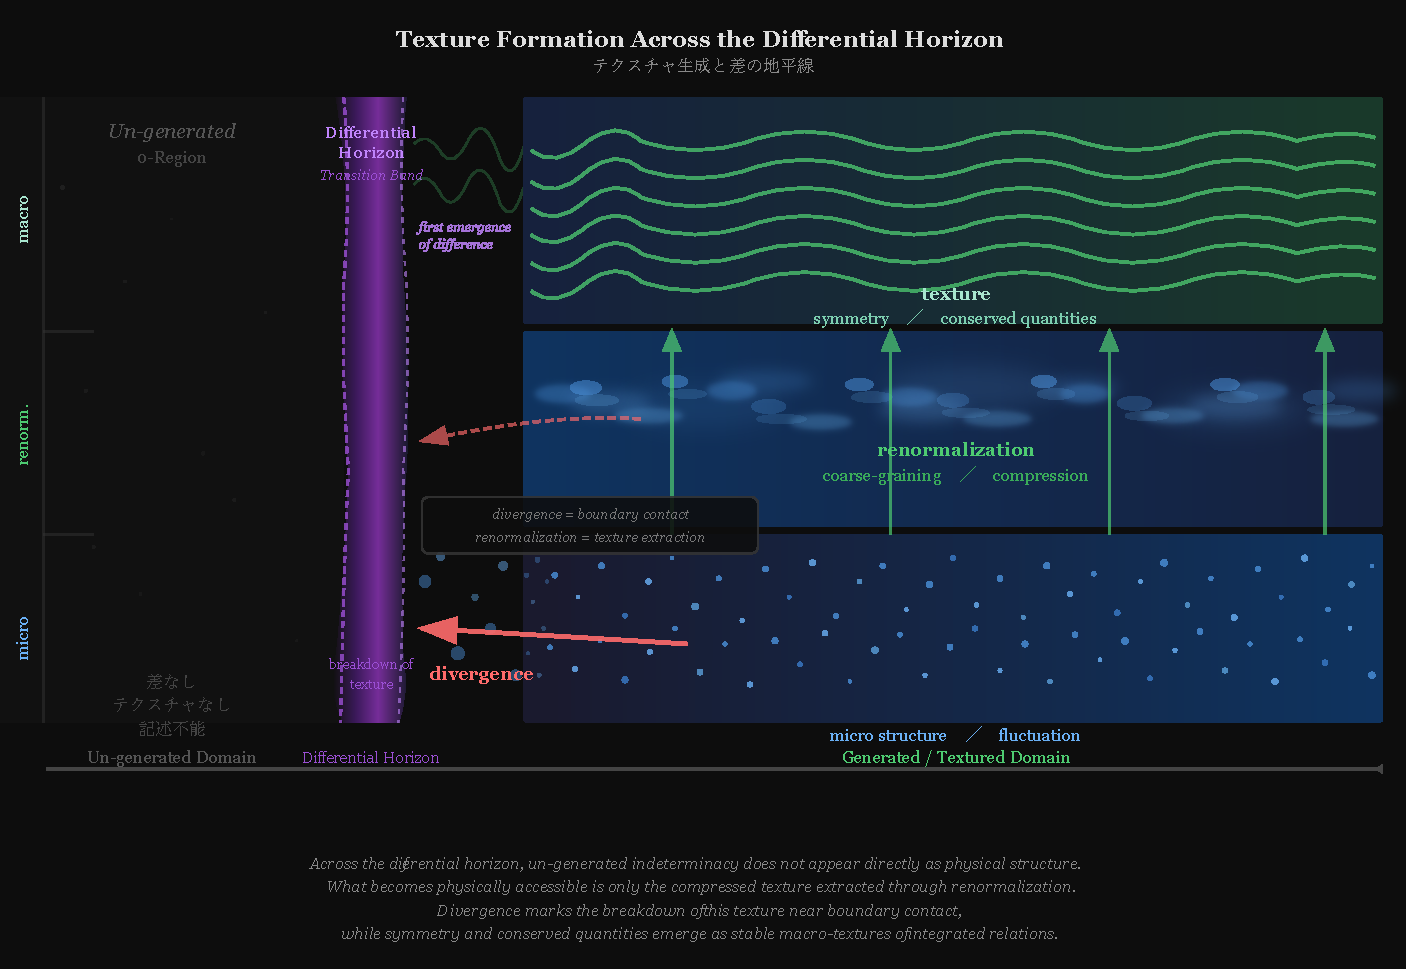
\includegraphics[width=\linewidth]{figures/figure1_texture_horizon.pdf}
  \caption{%
    Texture formation across the \DH{}.
    The \ungenerated{} domain (left) contains no difference, no structure,
    and no describable form.
    The transition band (center) is the \DH{}.
    The \generated{} domain (right) is organized into three layers:
    micro-structure and fluctuation (bottom),
    renormalization and coarse-graining (middle),
    and stable texture, symmetry, and conserved quantities (top).
    Divergence marks the breakdown of texture near \bcontact{}.
    \textit{The world appears not as raw microstructure,
    but as compressed texture.}
  }
  \label{fig:texture_horizon}
\end{figure}

The next section examines how this approach occurs in concrete terms,
through two distinct modes:
spatial convergence and temporal convergence.
